
\begin{abstract}

\textbf{Background.} The international adoption of Chinese high-speed railway technology has increased demand for bilingual knowledge transfer and vocational training. Existing railway large language model studies often examine domain adaptation or retrieval-augmented generation separately, leaving limited evidence on how bilingual model adaptation, governed retrieval, evidence provenance and resource-constrained deployment interact. This study therefore investigates knowledge-enhanced large language models and implements a bounded artificial intelligence agent system as a controlled experimental and application environment for international learners and vocational trainees, railway technical and service professionals, and personnel engaged in training, consulting and management.

\textbf{Methods.} An expert-governed bilingual railway corpus was organised with pair-grouped controls to separate training, validation and held-out evaluation records. Qwen2.5-7B and GLM-4-9B were evaluated before and after bilingual QLoRA adaptation, with Qwen3-14B retained as a reference. BM25, BGE-M3 dense retrieval and reciprocal-rank-fusion hybrid retrieval were compared on 400 held-out knowledge pairs; no-retrieval and retrieval-augmented generation were evaluated on 1,526 held-out bilingual question-answer examples. The evaluation covered Evidence Recall@k, mean reciprocal rank, Answer F1, paired significance, evidence support and resource use under single-machine deployment.

\textbf{Results.} Hybrid retrieval achieved Evidence Recall@5 of 0.715 in Chinese and 0.708 in English, exceeding the strongest single-retriever results of 0.690 and 0.685, respectively; the bilingual-field index attained the highest balanced mean of 0.696. Qwen QLoRA increased held-out Answer F1 from 0.189 to 0.398 in Chinese and from 0.437 to 0.648 in English, with both gains remaining significant after Holm correction. Under hybrid retrieval-augmented generation, it achieved the highest Answer F1 of 0.660 and 0.651, exceeding the Qwen3-14B reference values of 0.442 and 0.454. All evaluated generator conditions completed within the defined single-machine resource boundary.

\textbf{Conclusion.} Combining bilingual parameter-efficient adaptation with governed hybrid retrieval improves cross-language evidence access and domain question answering while remaining feasible under resource-constrained single-machine deployment. The model-centred framework provides a transferable approach for jointly evaluating adaptation, retrieval and evidence governance, and offers a locally controlled foundation for bilingual railway education and international workforce development.

\textbf{Keywords:} knowledge-enhanced large language models; bilingual domain adaptation; retrieval-augmented generation; evidence-conditioned generation; railway vocational education; resource-constrained deployment; bounded artificial intelligence agents; Web information systems

\end{abstract}
\section{Introduction}

Railway vocational education combines safety-critical regulations, specialised terminology and procedural textbook knowledge. International learners, vocational trainees and railway personnel working across languages must often move between Chinese source material and English learning support. Generic large language models can produce fluent answers, but their parametric knowledge does not expose a stable boundary between verified railway knowledge and unsupported generation. This is a Web information-system problem as much as a model problem: knowledge must be acquired, governed, retrieved, presented and traced to its source within an explicitly bounded local runtime.

The problem has practical importance beyond classroom convenience. China's high-speed railway development has generated international interest in its engineering and organisational experience, while railway internationalisation has also created an education and skills-transfer agenda \citep{lawrence2019hsr,xu2018education}. The intended users therefore extend beyond enrolled students to locally employed staff, technical specialists, service personnel, trainers, consultants and managers. This study does not claim that one system resolves the wider training gap; it addresses the narrower need for locally controlled bilingual access to reviewed railway knowledge. Such a service must do more than translate isolated terms: it must connect a bilingual question to an admissible regulation or teaching passage, preserve provenance and expose review state. Transportation studies have explored specialised language models for safety, rail design, track management, prognostics, driver advice and interactive railway training \citep{zheng2023trafficsafety,lahnalampi2024rail,wang2024phm,song2025railway,luo2025driver,li2025training}, while broader reviews identify reliability and deployment as continuing challenges \citep{wandelt2024transport}. Bilingual access, governed evidence and reproducible local deployment nevertheless remain under-examined as a combined information-system problem.

The hardware condition is defined operationally rather than inferred from an unverified claim about most institutions. Resource-constrained deployment in this study means one commercially available workstation with an RTX 3090 24 GB GPU and 32 GB host memory, without a multi-GPU cluster or a required paid-cloud inference path. The term comparatively low-cost refers to this single-machine topology and avoidance of continuing cluster or cloud dependence; it is not a market-price or total-cost-of-ownership estimate. This definition supports reproducibility and follows the broader call to report computational efficiency alongside model quality \citep{schwartz2020green}. Parameter-efficient adaptation and quantisation make this profile feasible \citep{dettmers2023qlora,ding2023peft,lv2024full,wang2025peft}, but lower trainable-parameter counts do not themselves demonstrate acceptable runtime memory or latency.

Existing studies commonly evaluate either general-purpose language models or retrieval-augmented generation in isolation. Four gaps motivate this work. First, bilingual educational retrieval is rarely evaluated separately by query language. Second, expert review is often described as preprocessing rather than implemented as a queryable governance state. Third, domain adaptation is frequently evaluated only on the target task, leaving translation regressions and citation-following failures hidden. Fourth, the term agent is often used without defining its action boundary, while deployment reports may omit the interaction between retrieval quality, answer traceability and measured single-workstation cost.

This study addresses the following research questions:

\begin{itemize}
\item \textbf{RQ1:} How accurately do BM25, pgvector dense retrieval and hybrid fusion retrieve evidence-equivalent indexed records for held-out Chinese and English railway question-answer pairs?
\item \textbf{RQ2:} How do retrieval strategies affect answer overlap and citation-format compliance, and can approved-only record eligibility be enforced and audited at retrieval time?
\item \textbf{RQ3:} What bilingual translation quality is achieved in each direction, and how does completion-only QLoRA affect domain QA without contaminating the held-out test set?
\end{itemize}

The study makes four contributions. First, it operationalises a bilingual railway knowledge base in which review state, source metadata, language variants and revision history remain queryable rather than being flattened into an anonymous vector collection. Second, it develops a bounded PostgreSQL/pgvector agent workflow that combines lexical and multilingual dense retrieval with evidence-labelled local generation while keeping retrieval policy operator-configurable. Third, it introduces a pair-grouped protocol that separates Chinese and English retrieval, QA and translation outcomes and states the remaining duplicate-evidence boundary explicitly. Fourth, it evaluates adaptation, retrieval and inference jointly on the defined single workstation, exposing both quality gains and failures in citation following, directional translation and runtime resource use.

\section{Related work}

\subsection{Knowledge-enhanced Web information systems}

Web information systems increasingly combine structured data management, semantic access and generative interfaces. Work in \emph{International Journal of Web Information Systems} shows the value of integrating knowledge representation, process state and user-facing tasks rather than treating them as isolated technical components \citep{hubscher2021knowledge}. Retrieval-augmented generation (RAG) provides a practical separation between parametric generation and an externally maintained evidence collection \citep{lewis2020rag}. This separation is relevant to institutional knowledge systems because source records can be revised without retraining the generator. It does not, however, guarantee faithful generation: retrieval can miss relevant evidence, and a generator can still misrepresent correctly retrieved material. The present study therefore evaluates retrieval, answer overlap, evidence support and citation-format behaviour as distinct outcomes.

The retrieval layer combines complementary lexical and semantic signals. BM25 remains an efficient lexical baseline for exact domain terms \citep{robertson2009bm25}, while reciprocal-rank fusion can combine rankings without requiring directly comparable score scales \citep{cormack2009rrf}. PostgreSQL and pgvector place vector search beside governed relational metadata, allowing approval state and held-out split boundaries to be applied in the query rather than after generation. This makes knowledge governance an executable part of the information-system design.

This distinction separates the proposed system from a document-only RAG demonstration. A Web information system must maintain record identity and lifecycle state across ingestion, review, retrieval and presentation. In this study the vector representation is derived data attached to a governed record, not the primary source of truth. Deleting, revising or withholding a record can therefore change retrieval eligibility without rebuilding the entire application or relying on prompt instructions to enforce governance.

\subsection{Retrieval-augmented generation in education}

Generative AI can support explanation, feedback and access to learning resources, but education research has also identified risks involving factual reliability, learner over-reliance and opaque provenance \citep{kasneci2023chatgpt,unesco2023guidance}. Survey evidence from legal-document question answering similarly shows that specialised LLM services require coordinated data processing, model adjustment and application frameworks rather than model substitution alone \citep{yang2024legalqa}. Educational RAG addresses part of this problem by conditioning responses on course or institutional material. Many demonstrations nevertheless report a pooled answer score without isolating retrieval failure, language effects or deployment cost. Such aggregation is particularly problematic for international vocational education, where an English query may need evidence originating in Chinese regulations or textbooks. This study consequently reports Chinese and English retrieval and generation separately and preserves document-level provenance in every retrieved result.

Railway applications illustrate why this separation matters. RSChat addresses railway safety question answering \citep{li2024rschat}, and an LLM-based human-computer training assistant has been evaluated for railway dispatching, education and professional training \citep{li2025training}. Domain-specialised systems have also been proposed for train-driver advice and emergency-response generation \citep{luo2025driver,huang2026emergency}. These studies establish the value of domain knowledge and training support, yet the present operational target differs: a bilingual user may formulate a concept in English, require Chinese-source evidence and need visible provenance and review state. The present work therefore evaluates cross-language access, governance and a defined single-workstation deployment together.

\subsection{Bounded agents and resource-aware deployment}

Classical agent research associates agency with situated action and a degree of autonomy \citep{wooldridge1995agents}, while recent LLM-agent surveys describe planning, memory, tool use and environmental action as common but variable components \citep{xi2025agents}. The present system uses the term \textbf{bounded workflow agent} in a narrower, operational sense. Its fixed action space is to route Chinese or English fields, invoke an operator-selected BM25, vector or hybrid retriever, enforce record eligibility, assemble numbered evidence, call a local generator and return a deterministic no-evidence or retrieval fallback. It does not set open-ended goals, browse the external Web, select arbitrary tools or change the knowledge base without human approval. Retrieval mode and top-\emph{k} remain user- or operator-configured. This boundary distinguishes the implemented service from an autonomous general-purpose agent and makes each action auditable.

Resource-aware evaluation is part of that boundary. Efficient-AI research argues that computational cost and efficiency should be reported alongside predictive quality \citep{schwartz2020green}. For a local agent, a small adapter file or a low trainable-parameter percentage does not establish low inference memory or latency. The present study therefore treats the defined workstation, peak reserved GPU memory, generation speed and latency as reproducibility conditions rather than inferring affordability from parameter count alone.

\subsection{Bilingual domain adaptation and evaluation}

Bilingual domain systems require both cross-lingual retrieval and controlled generation. BGE-M3 supports multilingual dense retrieval and was selected to provide a shared embedding space for the Chinese and English knowledge fields \citep{chen2024bgem3}. Dense similarity is not assumed to dominate lexical matching; the two methods are compared independently before fusion.

Parameter-efficient adaptation provides a second mechanism for domain specialisation. QLoRA trains low-rank adapters through a frozen 4-bit quantised base model, reducing memory requirements while retaining task adaptation capacity \citep{dettmers2023qlora}. In this study, completion-only masking prevents the prompt from contributing to the training loss, and bilingual variants sharing a knowledge-pair identifier remain in the same split. Translation is evaluated directionally because Chinese-to-English and English-to-Chinese scores are not interchangeable. Terminology and complete-sentence translation are also kept separate.

PEFT methods reduce trainable parameters but do not guarantee a better deployed system \citep{ding2023peft,wang2025peft}. Limited-resource training remains sensitive to quantisation, sequence length, optimiser state and model-specific target modules \citep{lv2024full}. Moreover, task adaptation can improve answer overlap while degrading factuality, instruction following or unrelated capabilities \citep{tian2024factuality,barnett2024finetuning}. This motivates the present before-and-after design, which reports not only domain QA but also general-capability checks, citation behaviour and memory use.

The frontier is consequently shifting from demonstrating that a domain large language model can generate an answer to establishing whether a knowledge-enhanced workflow can be adapted, governed and served locally within bounded compute and memory. This systems perspective requires joint reporting of model quality, retrieval quality, traceability, latency and peak memory; parameter efficiency alone is not a deployment result \citep{ding2023peft,lv2024full,wang2025peft}.

Domain translation creates a further risk of pooled evaluation. Prior work shows that fine-tuning effects depend on training direction, domain composition and data volume \citep{hu2024translation,vieira2024translation,zheng2024translation}. Consequently, this study does not interpret a single bilingual mean as evidence of robust translation. It reports terminology and sentence tasks independently in both directions and retains empty or wrong-language outputs as failures rather than silently discarding them.

\subsection{Research gap and analytical framework}

The literature suggests that domain retrieval, adaptation and local deployment are individually feasible, but it does not establish that their benefits compose monotonically or remain practical under a reproducible single-workstation constraint. The analytical framework therefore treats the system as four testable layers: governed knowledge, retrieval, generation/adaptation and deployment. A failure at one layer cannot be compensated for statistically by a high score at another. Evidence-equivalent retrieval recall is measured before answer generation; citation-format compliance is separated from answer overlap; translation is separated from QA; and quality is reported alongside latency and memory. This layered design provides the basis for answering RQ1-RQ3 without attributing every observed change to the language model alone.

\section{System design and research method}

\subsection{Application context and requirements}

The target users comprise four role groups. First, learners include international students, vocational trainees and Chinese-speaking learners requiring bilingual support. Second, railway practitioners include service personnel, locally employed staff and technical specialists in cross-border railway settings. Third, education and advisory users include vocational teachers, workplace trainers and technical consultants. Fourth, management and system-administration users include training managers and platform administrators. Figure 1 groups these four roles into three access clusters: learners and practitioners use the bilingual portal; teachers, trainers and consultants use the review console; managers and administrators use the operations console. The system must return concise answers, expose numbered evidence, preserve document metadata and run on the defined workstation without required cloud inference.

Figure 1 organises the online system into four layers. The user-and-role layer provides bilingual question answering, knowledge editing and review, and operational monitoring through the three access clusters. The Web-application layer presents search, conversation, evidence inspection and governance functions. The bounded-agent layer executes the fixed workflow defined in Section 2.3: language-field routing, operator-configured retrieval, eligibility filtering, rank fusion where selected, evidence assembly, local generation and deterministic fallback. The local-infrastructure layer hosts the model, embedding service and governed PostgreSQL store. Together, the layers serve three purposes: bilingual access, inspectable evidence and reproducible operation on one workstation.

Figure 2 complements this runtime view with a four-stage governance and evaluation lifecycle. Source acquisition and bilingual editing create candidate records; expert review assigns approval, revision or rejection state; approved records enter the production BM25 and vector indexes; and pair-grouped split controls isolate the exact held-out question-answer records from both production indexes and QLoRA training. Retrieval evaluation can still match another admissible indexed record containing equivalent evidence, as defined in Section 3.5. Learners and practitioners consume approved evidence, teachers, trainers and consultants review and revise domain content, and managers and administrators supervise versions, audit events and resource status. These mappings produce five design requirements: bilingual access, source traceability, review-state enforcement, explicit evaluation isolation and single-workstation reproducibility.

\subsection{Expert-governed knowledge base}

Knowledge records include Chinese and English questions and answers, evidence, original text, source document, chapter, page, task type, quality flags, review status and revision history. PostgreSQL stores governed records; pgvector stores 1,024-dimensional BGE-M3 embeddings. The production index excludes the exact records assigned to the held-out test split.

The knowledge sources comprise railway terminology, operating and safety regulations, and vocational textbook or concept material. Ingestion preserves source-document, chapter and page fields whenever available. Chinese and English questions and answers are stored in separate fields on the same logical record so that a language variant does not lose its source identity. Embeddings are linked by record identifier and model revision; they can be rebuilt without changing the reviewed text. A record marked \texttt{rejected}, \texttt{needs\_revision} or as part of the frozen RAG test is excluded before ranking. This database-level decision prevents the exact test record from leaking through BM25 or vector retrieval. It does not prove that semantically equivalent evidence is absent from every other record, which is why the retrieval outcome is defined as evidence-equivalent recall rather than exact-record recall.

The three authors jointly constructed and checked the knowledge base and the training and evaluation datasets; their combined expertise covers railway vocational education, international vocational education, environmental and data analysis, and software and multimodal language-model engineering. The released governance audit, however, contains only two distinct reviewer identifiers. The paper therefore reports two auditable reviewer accounts and does not reinterpret author-level checking outside those identifiers as a third independent review pass. Because this was an author-led governance procedure rather than an independent inter-rater study, no inter-rater agreement statistic or external expert consensus is claimed. \texttt{Approved} is analysed only as an executable eligibility state.

Figure 2 distinguishes the authoritative PostgreSQL record from its derived BM25 and pgvector indexes across the four lifecycle stages introduced in Section 3.1. Approval, revision and rejection are written back as review state and audit events; a revision returns to bilingual editing rather than restarting source acquisition. Pair-grouped split metadata isolates the held-out test branch from production indexes and QLoRA training.


\begin{figure}[ht]
\centering
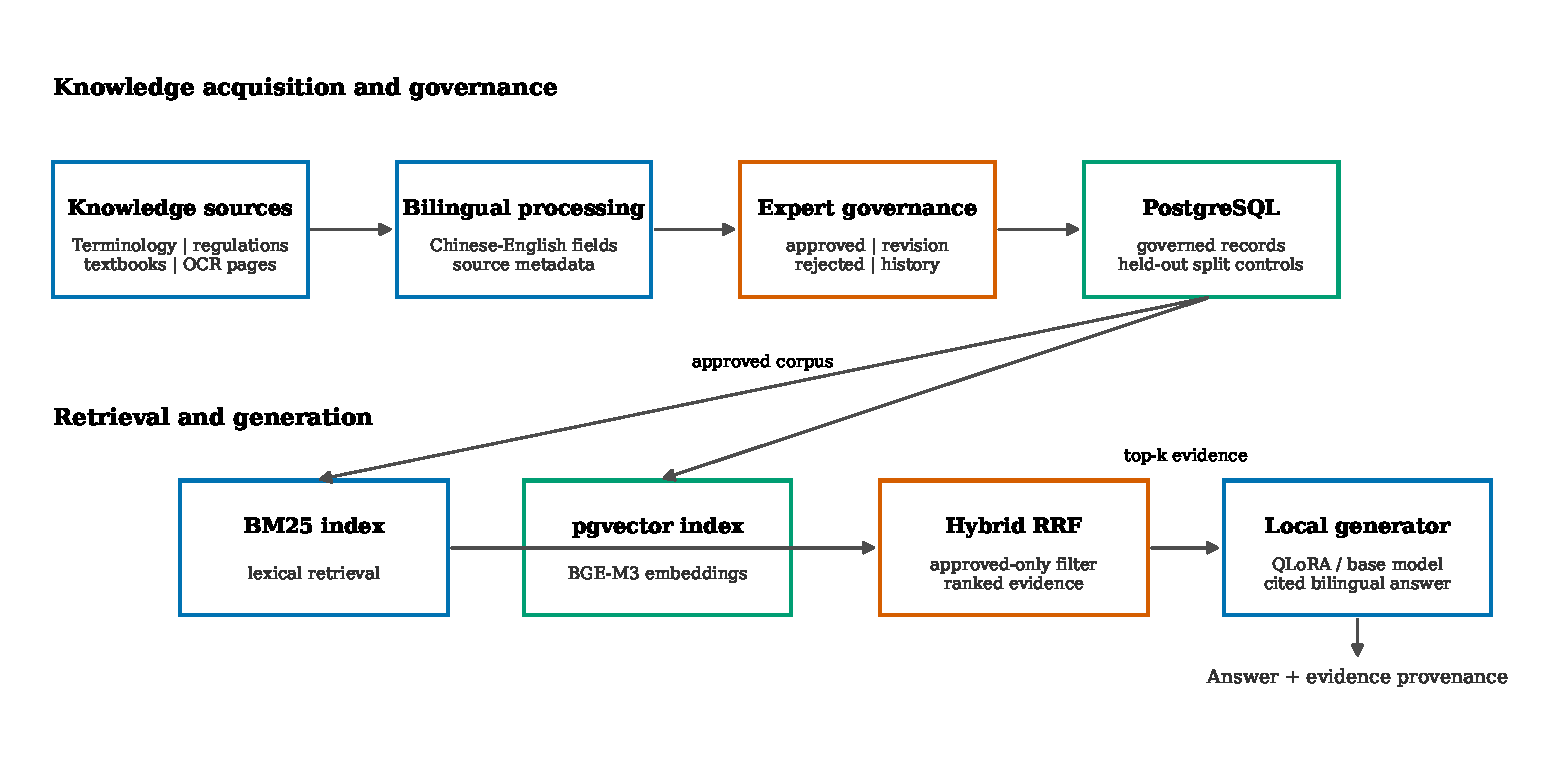
\includegraphics[width=0.96\linewidth,keepaspectratio]{../paper/ijwis/figures/system_architecture.pdf}
\caption{Four-layer bounded bilingual agent workflow linking three role-access clusters to Web applications, governed retrieval, local generation and single-workstation infrastructure. Solid arrows denote runtime or data flow; dashed arrows denote governance or control. Source: Authors' own work.}
\end{figure}


\begin{figure}[ht]
\centering
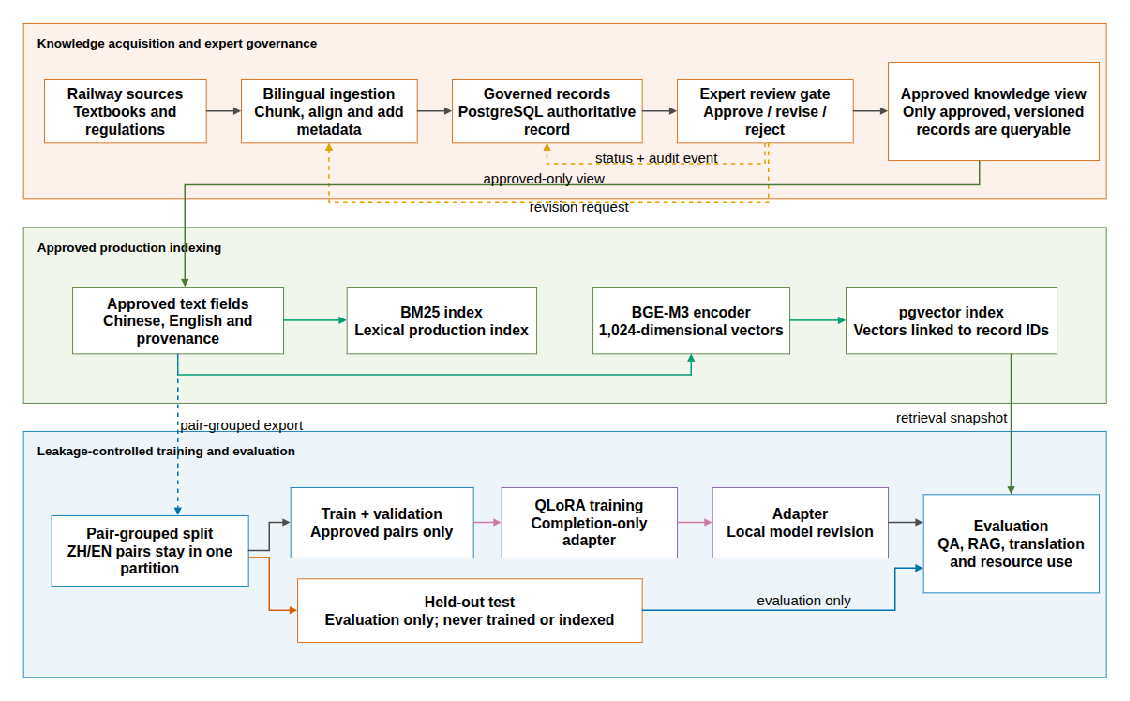
\includegraphics[width=0.96\linewidth,keepaspectratio]{../paper/ijwis/figures/knowledge_governance_lifecycle.pdf}
\caption{Expert-governed knowledge, production-index and evaluation lifecycle with exact held-out records excluded from indexing and training. Source: Authors' own work.}
\end{figure}

\subsection{Retrieval and answer generation}

BM25 indexes Chinese and English question-answer fields and evidence. Dense search embeds a query with BGE-M3 and ranks chunks by vector similarity. Hybrid retrieval fuses keyword and dense rankings using reciprocal-rank fusion. The \texttt{approved\_only} condition applies review status as a database-level eligibility filter. Retrieval mode and top-\emph{k} are configured by the user or operator rather than selected autonomously by the language model. Retrieved evidence is numbered and supplied to the local generator with an instruction to answer in the query language and cite evidence labels.

Following Cormack \emph{et al.} (2009), the reciprocal-rank-fusion score for a candidate document \emph{d} is defined in Equation (1):

\begin{equation}
\operatorname{RRF}(d)=\sum_{r \in \{\mathrm{BM25},\mathrm{vector}\}}\frac{1}{k_0+\operatorname{rank}_r(d)}.
\end{equation}

In Equation (1), a document absent from a retriever's candidate list contributes zero for that retriever. The candidate pool is fixed at 50 per retriever and the conventional rank constant is \texttt{k0 = 60}; Equation (1) is applied before final top-\emph{k} is varied. This controlled top-\emph{k} comparison changes the amount of evidence delivered to the generator without changing the upstream search pool. Dense ranking uses BGE-M3 query embeddings and pgvector distance, while lexical ranking retains exact matches that are valuable for abbreviations, equipment names and regulation numbers. Every returned evidence object contains record identifier, source document, task type and retrieval score.

The FastAPI service exposes search and conversational endpoints to the Web client. At answer time, the selected evidence is serialised with labels such as \texttt{[Evidence1]} or \texttt{[证据1]}. The system instruction requires the generator to answer in the query language, remain within the supplied evidence and attach labels to supported statements. If no admissible record is retrieved, the workflow returns an explicit no-evidence message; if generation fails, it returns the highest-ranked source as a retrieval fallback. These fixed actions constitute the bounded agent policy. The output is described as evidence-conditioned rather than inherently grounded because citation-format compliance and semantic support are evaluated separately.

\subsection{Bilingual QLoRA adaptation}

The adaptation dataset is generated only from approved records and split by knowledge-pair identifier, task type and source document. Chinese and English variants of the same knowledge item are assigned to the same partition. The current frozen 80/10/10 corpus contains 12,178 training, 1,524 validation and 1,526 test examples, balanced equally by language, with zero knowledge-pair identifier overlap among partitions. The 120 regulation items reserved for RAG evaluation are forced into the test partition and never used for training. Pair-level isolation does not establish the absence of exact or near-duplicate evidence under different record identifiers; this unmeasured boundary is retained in the interpretation. Loss is computed only on answer tokens; all prompt labels are masked with \texttt{-100}.

Qwen2.5-7B-Instruct and GLM-4-9B-Chat-HF form the adaptation matrix; their architectures and post-training lineage are documented in the corresponding official technical reports \citep{qwen2024technical,glm2024chatglm}. Both were loaded with NF4 quantisation and PEFT adapters on the target GPU. Qwen exposes separate \texttt{gate\_proj} and \texttt{up\_proj} modules, whereas GLM uses a fused \texttt{gate\_up\_proj}; model-specific target lists are therefore required. The formal rank-64 configuration trained 161,480,704 Qwen parameters and 190,382,080 GLM parameters, representing 3.58 and 3.45 per cent of the parameters visible to the quantised training process, respectively. Qwen3-14B is retained only as an unadapted reference generator and is associated with the Qwen3 technical report \citep{qwen2025technical}.

Both runs use LoRA rank 64, alpha 16, dropout 0.05, learning rate \texttt{2e-4}, maximum sequence length 1,024 and one epoch. The per-device batch size is one with 16 gradient-accumulation steps and a 0.03 warm-up ratio. Random seed 42 is fixed in the experiment configuration. Generation uses greedy decoding (\texttt{temperature = 0}, \texttt{top\_p = 1}) with a task-dependent output limit. Completion-only supervision masks every prompt token with \texttt{-100}; therefore, training optimises the answer sequence rather than teaching the model to reproduce instructions. This choice is tested rather than assumed to improve every downstream behaviour.

\subsection{Evaluation design}

Retrieval conditions are BM25, vector, hybrid and approved hybrid. Metrics are evidence-equivalent Recall@1/3/5, MRR and mean latency. The formal generator matrix fixes no retrieval, BM25-RAG and approved hybrid-RAG so that five generators receive identical cached contexts. Automatic metrics include Answer F1, reference containment, citation-format coverage, citation omission and end-to-end latency. Citation measures are treated as instruction-following indicators, not evidence entailment or factual hallucination measures. Translation is reported independently for Chinese-to-English and English-to-Chinese terminology and sentences using SacreBLEU, chrF++ and COMET (\texttt{Unbabel/wmt22-comet-da}). This multi-dimensional protocol follows the broader principle that LLM evaluation should separate task capability, robustness and deployment behaviour rather than rely on one aggregate score \citep{chang2024survey}.

Evidence-equivalent Recall@\emph{k} is one when at least one of the first \emph{k} candidates satisfies the frozen matching rule: the same record identifier, normalised gold and candidate evidence containment in either direction, or the same source document with the gold answer contained in candidate evidence. Because exact RAG-test records are excluded from the production index, observed hits normally arise from the latter evidence-equivalence criteria rather than identity. MRR averages the reciprocal rank of the first such match. Character-level F1 is used for Chinese and token-normalised F1 for English. Reference containment records whether the normalised reference appears in the generated answer. Citation-format coverage records only whether the requested evidence-label syntax appears; its complement is reported as citation omission. Neither measure tests claim-evidence entailment or factual hallucination.

All core comparisons use paired samples. Mean metrics are accompanied by 2,000-resample bootstrap 95 per cent confidence intervals in the released analysis tables. Original-versus-QLoRA comparisons use two-sided paired Wilcoxon tests, Cohen's \emph{d}\textsubscript{z} for paired effects and Holm correction across the pre-specified family recorded in the analysis configuration. Exploratory error categories are reported separately and are not treated as confirmatory hypothesis tests. Efficiency measurements use 30 Chinese short questions, 30 English short questions and 30 regulation-oriented long-context questions, with one warm-up and three measured repetitions per model condition.

Three automated system checks extend the primary protocol without introducing new human labels. First, source-only, Chinese-field, English-field and bilingual-field indexes are compared on the same 800 queries with a 512-token BGE-M3 window. Second, each of 8,000 RAG answers is segmented into claims; BGE-M3 cosine similarity estimates semantic support against all retrieved evidence and explicitly cited evidence at a pre-specified 0.45 threshold. This is a support proxy, not textual entailment or expert correctness. Third, immutable review events and before-state snapshots are audited for action and changed-field coverage. Generator resource behaviour is reported from the separate 270-measurement inference experiment for each condition.

\subsection{Implementation and reproducibility}

The application uses a Vite-based Web client, a FastAPI backend and PostgreSQL 16.14 with pgvector 0.8.4. Experiments ran on Linux with one NVIDIA GeForce RTX 3090 (24,576 MiB), 32 GB host memory, Python 3.11.15, PyTorch 2.11.0, Transformers 5.12.1, PEFT 0.18.1 and bitsandbytes 0.49.2. No multi-GPU or cloud inference resource is required by the evaluated path. This is the paper's reproducible single-workstation constraint and its comparative low-cost system profile; no purchase-price or total-cost claim is made. Qwen2.5-7B-Instruct, GLM-4-9B-Chat-HF and BGE-M3 are pinned by model revision in the frozen manifest. COMET uses the pinned \texttt{Unbabel/wmt22-comet-da} checkpoint. Input datasets, configurations, generated tables and final analysis assets are recorded with SHA-256 hashes. Table I summarises the formal implementation and experimental environment.

\begin{table}[ht]
\centering
\caption{Formal implementation and experimental environment.}

\begin{tabular}{p{0.28\linewidth}p{0.64\linewidth}}
\toprule
Component & Formal setting \\
\midrule
Database & PostgreSQL 16.14; pgvector 0.8.4 \\
Embedding & BAAI/bge-m3; 1,024 dimensions \\
Adapted generators & Qwen2.5-7B-Instruct; GLM-4-9B-Chat-HF \\
Reference generator & Qwen3-14B through Ollama 0.19.0 \\
Training & NF4 QLoRA; rank 64; one epoch; seed 42 \\
Hardware boundary & One RTX 3090 24 GB; 32 GB RAM; no multi-GPU or required cloud inference \\
Statistical analysis & 2,000 bootstrap resamples; paired Wilcoxon; Cohen's \emph{d}\textsubscript{z}; Holm correction \\
\bottomrule
\end{tabular}
\end{table}

The code separates test-set construction, embedding, retrieval evaluation, generator evaluation, adaptation and report export. This prevents an analysis script from silently changing the production index or training split. Cached retrieval contexts are reused across generators in the formal RAG matrix, so model comparisons receive identical evidence. The manifest records the Git state and every input hash at freeze time, supporting result reconstruction and consistent comparison across runs.

Production embedding loading is local-files-only by default, preventing an unavailable model registry from becoming a hidden runtime dependency. The real review and question-answering views were rendered through the running Vite and FastAPI services rather than reconstructed as mock-ups. The fixed environment, model revisions, split statistics and asset hashes allow reconstruction of the reported single-workstation comparisons.

\section{Results}

\subsection{Knowledge-base composition}

The database contains 37,661 approved records and 37,109 complete bilingual records. After freezing the formal RAG test, 37,261 approved non-test knowledge chunks have BGE-M3 embeddings. The QLoRA test partition contains 763 knowledge pairs across four source documents. From this partition, the formal cross-source RAG set contains 400 knowledge pairs and 800 language-specific queries: 150 regulation, 127 terminology and 123 textbook/concept pairs across 17 task types. The earlier 120-pair regulation pilot is a subset of this formal set and remains available in the reproducibility artifacts; it is not reported as an additional sample in the main results.

\subsection{Formal cross-source bilingual retrieval}

\begin{table}[ht]
\centering
\caption{Formal cross-source evidence-equivalent retrieval on 400 knowledge pairs.}

\small
\begin{adjustbox}{max width=\linewidth}
\begin{tabular}{>{\raggedright\arraybackslash}p{0.19\linewidth}lrrrrr}
\toprule
Retrieval & Language & Evidence R@1 & Evidence R@3 & Evidence R@5 & MRR & Mean latency (ms) \\
\midrule
BM25 & Chinese & 0.520 & 0.595 & 0.620 & 0.560 & \textbf{69.5} \\
Vector & Chinese & 0.518 & 0.653 & 0.690 & 0.588 & 134.4 \\
Hybrid approved & Chinese & \textbf{0.570} & \textbf{0.675} & \textbf{0.715} & \textbf{0.628} & 217.6 \\
BM25 & English & \textbf{0.570} & \textbf{0.670} & 0.685 & 0.620 & \textbf{59.0} \\
Vector & English & 0.463 & 0.553 & 0.580 & 0.509 & 134.4 \\
Hybrid approved & English & \textbf{0.570} & 0.668 & \textbf{0.708} & \textbf{0.620} & 209.2 \\
\bottomrule
\end{tabular}
\end{adjustbox}
\end{table}

Table II reports the formal evidence-equivalent retrieval comparison. BM25 is particularly competitive for English terminology queries, while dense retrieval records higher Chinese evidence recall in this evaluation. With the RRF candidate pool fixed at 50 for every final cutoff, hybrid fusion obtains the highest Evidence Recall@5 in both languages, although its latency is approximately three times that of BM25. Increasing the final cutoff from three to eight raises hybrid evidence recall from 0.675 to 0.743 in Chinese and from 0.668 to 0.723 in English, while mean retrieval latency remains nearly constant in this controlled evaluation (Figure 3). Approved-only and unfiltered hybrid results are identical because all admissible indexed records in this frozen experiment satisfy the approval condition. These values concern the matching rule in Section 3.5; they must not be interpreted as retrieval of the excluded test record itself.


\begin{figure}[ht]
\centering
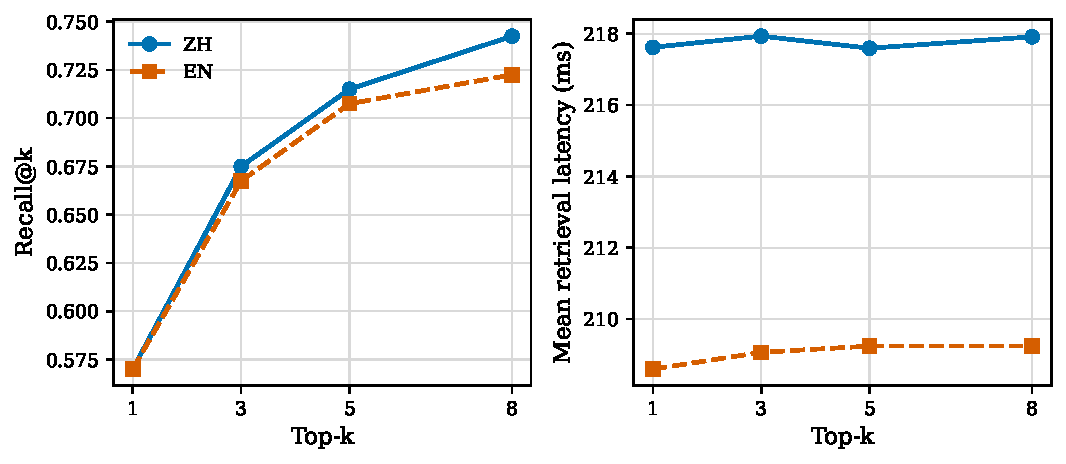
\includegraphics[width=0.96\linewidth,keepaspectratio]{../paper/ijwis/figures/top_k_quality_latency.pdf}
\caption{Hybrid evidence-equivalent retrieval quality and latency across top-k settings. Left: Evidence Recall@k; right: mean retrieval latency. Source: Authors' own work.}
\end{figure}

\subsection{QLoRA adaptation and held-out QA}

Both one-epoch training runs converged without interruption. Qwen trained for 3,546 s (59.1 min), with final training and validation losses of 0.950 and 0.720 and peak reserved memory of 13.0 GB. GLM trained for 4,571 s (76.2 min), with losses of 1.146 and 0.794 and peak reserved memory of 15.0 GB. The respective validation perplexities were 2.05 and 2.21.

Figure 4 presents the training and validation trajectories. Because each model was trained for one epoch, the curves establish completion and optimisation behaviour rather than convergence across repeated schedules. The absence of an extended hyperparameter search is consistent with the resource-constrained design but limits claims about globally optimal adapter settings.

On the 1,526-example held-out bilingual QA set, Qwen QLoRA increased Answer F1 from 0.189 (95 per cent CI 0.175-0.204) to 0.398 (0.376-0.422) in Chinese and from 0.437 (0.419-0.455) to 0.648 (0.632-0.664) in English. GLM increased from 0.192 to 0.410 in Chinese and from 0.498 to 0.552 in English. All four paired gains remained significant after Holm correction (all adjusted p-values below 0.01); Cohen's \emph{d}\textsubscript{z} was 0.569 and 0.634 for Qwen Chinese and English, and 0.614 and 0.146 for GLM. Qwen therefore provides the strongest balanced adapted QA result, while the small GLM English effect cautions against pooling languages. These sample-level tests do not estimate variation across repeated training seeds.

A limited general-capability check (maximum 200 examples per subtask) found that Qwen C-Eval/MMLU accuracy changed from 0.788/0.739 to 0.775/0.728, whereas GLM changed from 0.675/0.673 to 0.683/0.679. These small changes do not indicate broad catastrophic forgetting, but the limited protocol is a regression check rather than a comprehensive general benchmark.


\begin{figure}[ht]
\centering
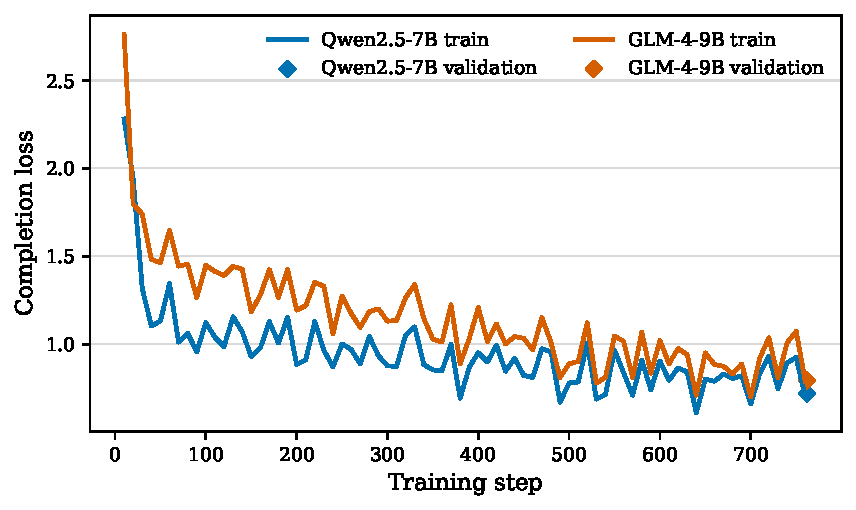
\includegraphics[width=0.96\linewidth,keepaspectratio]{../paper/ijwis/figures/training_validation_loss.pdf}
\caption{Completion-only QLoRA training and validation loss for Qwen2.5-7B and GLM-4-9B. Source: Authors' own work.}
\end{figure}

\subsection{Multi-generator RAG comparisons}

Approved-hybrid RAG significantly improved Answer F1 over no retrieval for every generator and language after Holm correction. The adjusted p-values for Chinese and English, respectively, were 1.89e-39 and 2.28e-42 for original Qwen, 1.13e-22 and 9.56e-31 for original GLM, 1.34e-06 and 1.41e-11 for Qwen QLoRA, 3.16e-09 and 9.37e-03 for GLM QLoRA, and 6.66e-32 and 7.58e-29 for Qwen3-14B. For original Qwen, F1 rose from 0.262 to 0.402 in Chinese and from 0.306 to 0.440 in English (paired effect sizes 0.796 and 0.798). Qwen QLoRA achieved the highest absolute RAG F1, 0.660 in Chinese and 0.651 in English, exceeding the Qwen3-14B reference values of 0.442 and 0.454. However, its incremental hybrid-RAG gains over no retrieval were only 0.030 and 0.078, compared with 0.141 and 0.133 for original Qwen. BM25 and hybrid did not have a uniform answer-quality ordering: original-Qwen BM25/hybrid F1 was 0.406/0.402 in Chinese and 0.433/0.439 in English, while Qwen-QLoRA values were 0.674/0.660 and 0.644/0.651. Similar rank reversals occurred for GLM and Qwen3. The observed answer-overlap gains therefore differed by adaptation, retrieval strategy and language.

The traceability result was different. For original Qwen, citation-format coverage moved from 0.543/0.638 under BM25 to 0.595/0.643 under hybrid in Chinese/English; Qwen3 moved from 0.715/0.900 to 0.788/0.905. By contrast, Qwen QLoRA achieved only 0.000/0.003 under hybrid, and GLM showed the same, less extreme adaptation-related pattern. In the tested conditions, QLoRA produced stronger answer overlap but weaker compliance with the citation instruction used in the evaluation targets; citation omission consequently approached one for the adapted models. This is an instruction-following failure, not a measured factual hallucination rate. For an operational workflow, Qwen2.5 QLoRA is the primary answer-quality model, while original Qwen or Qwen3 remains the safer traceability control until citation-aware adaptation is added.

\subsection{Directional translation}

Translation effects were direction- and task-dependent. Qwen COMET moved from 0.501 to 0.509 for Chinese-to-English terminology and from 0.610 to 0.614 for English-to-Chinese sentences, but fell from 0.656 to 0.599 for Chinese-to-English sentences and from 0.596 to 0.485 for English-to-Chinese terminology. Its lexical metrics show the same lack of uniform benefit: Chinese-to-English terminology chrF++ increased from 10.41 to 16.69, whereas sentence chrF++ fell from 47.43 to 31.28.

Figure 5 visualises the before-and-after COMET changes by direction and task. The opposing slopes show that the result cannot be summarised as a single improvement or regression.

GLM QLoRA is a clear failure case. Its sentence COMET dropped from 0.667 to 0.348 for Chinese-to-English and from 0.742 to 0.343 for English-to-Chinese; corpus BLEU was zero in both directions. Automated inspection found 2,168 empty outputs among 2,634 translation examples (82.3 per cent). This result does not support a general claim that QA-oriented completion-only adaptation improves translation. Terminology and sentence translation are therefore reported separately from QA evaluation.


\begin{figure}[ht]
\centering
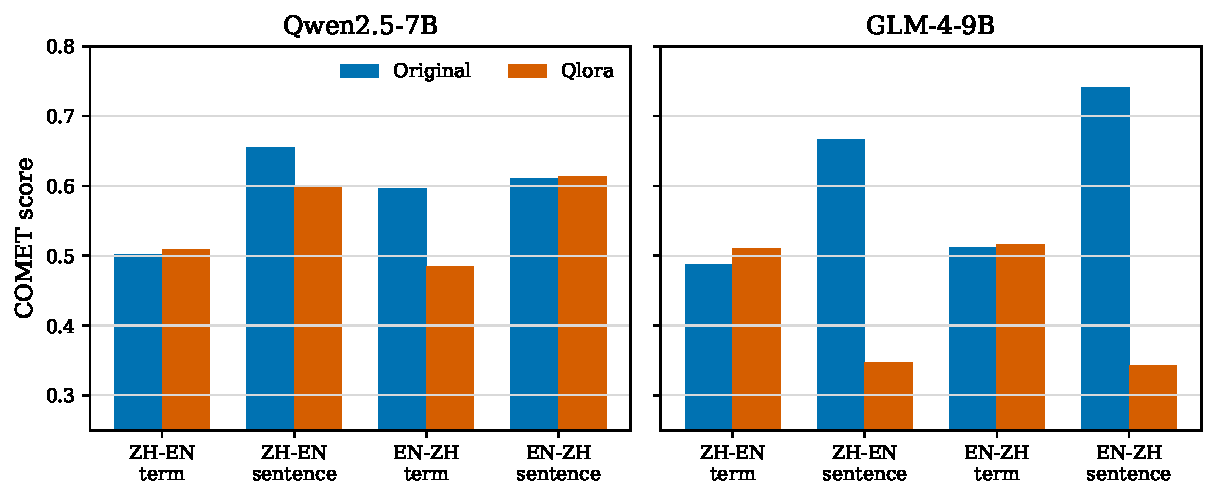
\includegraphics[width=0.96\linewidth,keepaspectratio]{../paper/ijwis/figures/translation_before_after.pdf}
\caption{Direction- and task-separated COMET before and after QLoRA. Left: Qwen2.5-7B; right: GLM-4-9B. Source: Authors' own work.}
\end{figure}

\subsection{Resource use and automated error analysis}

All five deployment conditions completed 270 measurements without failure or OOM. Original Qwen and GLM used 5.49 and 6.76 GB peak reserved memory and generated at 31.9 and 22.7 tokens/s. Their QLoRA variants used 16.11 and 19.49 GB and generated at 17.5 and 11.9 tokens/s. Qwen3-14B through Ollama used 14.26 GB and 78.5 tokens/s, although cross-backend timing should be interpreted cautiously. The Qwen and GLM adapters occupy approximately 627 and 746 MB. The low 2.63 s GLM QLoRA mean latency reflects abnormally short or empty outputs and is not an efficiency advantage. All configurations fit the target 24 GB workstation, but original Qwen provides the lowest resource cost and Qwen QLoRA the strongest QA quality within the limit.

The quality-latency-memory relationship is shown in Figure 6. The plot is interpreted as a deployment frontier rather than a universal model ranking because the Transformer and Ollama inference implementations use different backends.

Automated failure flags provide additional descriptive comparisons for the aggregate results. At top three, hybrid retrieval failed to return evidence satisfying the frozen equivalence rule for 32.5 per cent of Chinese and 33.3 per cent of English queries. Even with a hit, original Qwen produced low-overlap answers in 18.0 per cent of Chinese versus 4.3 per cent of English cases. Qwen QLoRA reduced these rates to 4.0 and 1.5 per cent, but omitted citation labels in 100.0 and 99.8 per cent. Figure 7 compares these automatically flagged categories. The translation analysis additionally exposed empty answers, wrong-language outputs and terminology substitutions. Near-duplicate evidence and citation entailment require separate semantic judgement and were not inferred from string-based flags.


\begin{figure}[ht]
\centering
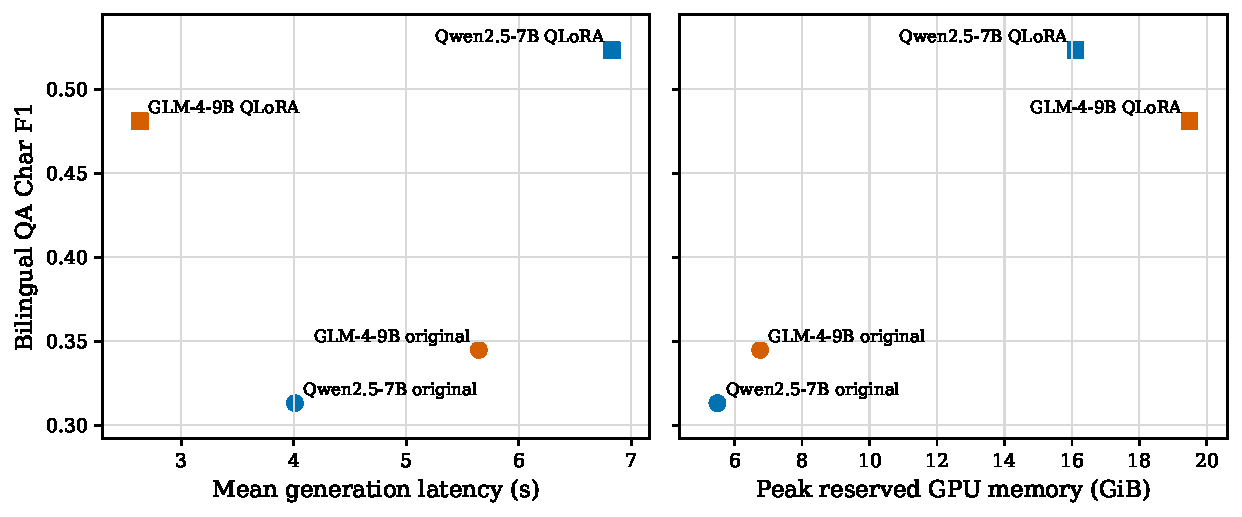
\includegraphics[width=0.96\linewidth,keepaspectratio]{../paper/ijwis/figures/quality_latency_pareto.pdf}
\caption{Bilingual QA quality against generation latency and peak GPU memory. Left: mean generation latency; right: peak reserved GPU memory. Source: Authors' own work.}
\end{figure}


\begin{figure}[ht]
\centering
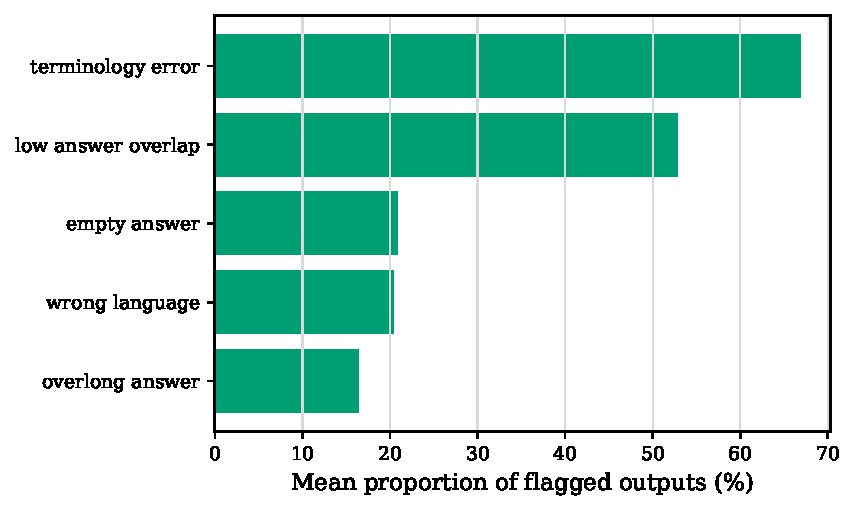
\includegraphics[width=0.96\linewidth,keepaspectratio]{../paper/ijwis/figures/error_type_distribution.pdf}
\caption{Mean prevalence of automatically flagged output errors across the evaluated generator and retrieval conditions. Source: Authors' own work.}
\end{figure}


\begin{figure}[ht]
\centering
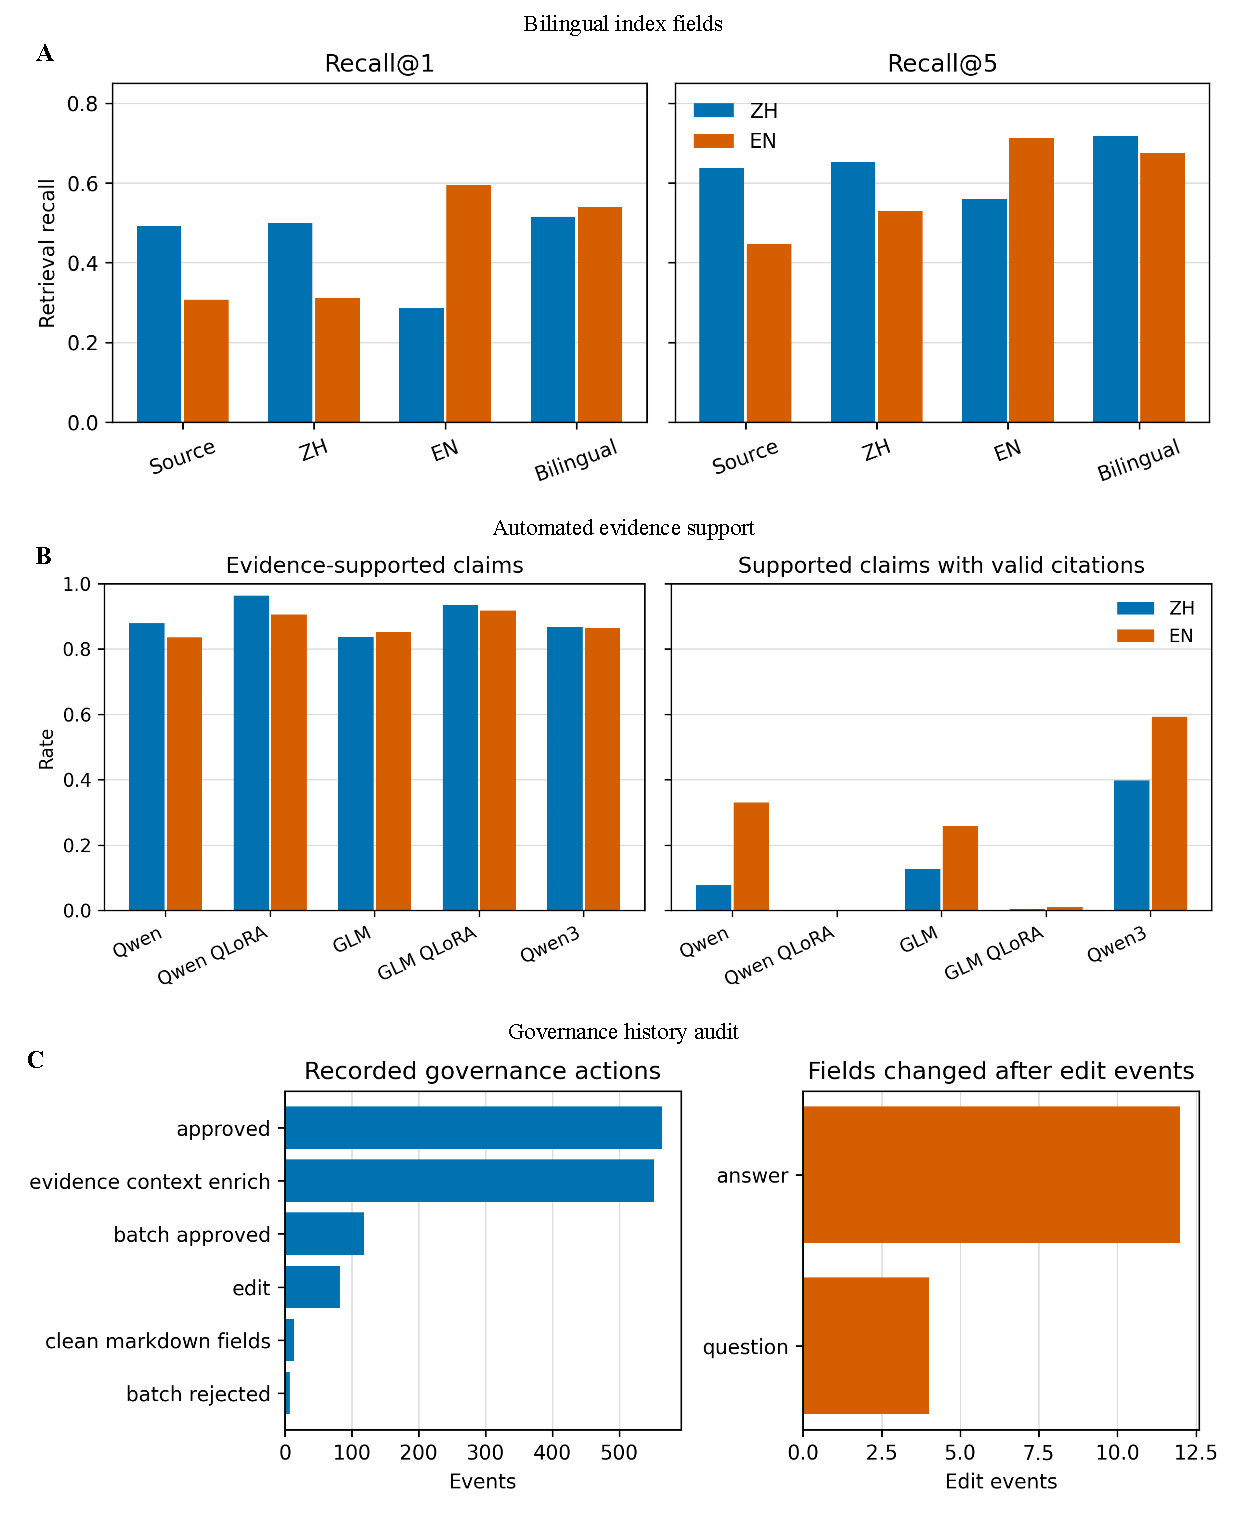
\includegraphics[width=0.96\linewidth,keepaspectratio]{../paper/ijwis/figures/supplementary_system_validation.pdf}
\caption{Bilingual index, automated evidence support and governance-history validation. Panels A-C report field ablation, evidence support and governance audit results, respectively. Source: Authors' own work.}
\end{figure}

\subsection{Index, evidence-support and governance validation}

\begin{table}[ht]
\centering
\caption{Supplementary information-system validation results.}

\begin{tabular}{p{0.38\linewidth}ccp{0.34\linewidth}}
\toprule
Validation & Chinese & English & Operational result \\
\midrule
Bilingual-field hybrid index, Evidence Recall@5 & 0.718 & 0.675 & Highest balanced mean (0.696) \\
Original Qwen hybrid, supported-claim proxy & 0.878 & 0.836 & Citation precision 0.955/0.970 \\
Qwen QLoRA hybrid, supported-claim proxy & 0.964 & 0.905 & Citation recall 0.000/0.002 \\
Governance history & - & - & 1,337 events; 82 edits; two recorded reviewers \\
\bottomrule
\end{tabular}
\end{table}

Table III reports three supplementary information-system validations. The field comparison reports different language-specific outcomes: English-only hybrid is strongest for English Evidence Recall@5 (0.713) but falls to 0.560 in Chinese, whereas the bilingual index gives the highest balanced mean. Across 27,668 segmented claims, hybrid retrieval generally records higher automated semantic support, but high support does not repair absent citations: Qwen QLoRA retains strong support scores while almost never attaching a valid label. The governance database contains 37,664 records and 1,337 review events, including before-state snapshots for edits; only three current records are rejected, so the experiment does not provide an approved-versus-rejected quality comparison. The audit exposes two distinct reviewer identifiers, consistent with the reporting boundary in Section 3.2. Figure 8 summarises these three checks.

\clearpage

\section{Discussion}

\subsection{Answers to the research questions}

\textbf{RQ1 concerned bilingual retrieval.} The evidence-equivalent comparison produced language-specific outcomes. Dense retrieval had higher recall in Chinese in this evaluation, whereas exact terminology made BM25 competitive in English. Hybrid fusion reached the highest Evidence Recall@5 in both languages, and the field comparison reported the strongest balanced result for the bilingual index even though an English-only index was best for English alone. Hybrid had higher latency, while lexical retrieval remained a credible lower-cost configuration. These conclusions apply to the pre-specified equivalence rule, not exact retrieval of records excluded from the index \citep{robertson2009bm25,cormack2009rrf}.

\textbf{RQ2 concerned retrieval strategy, enforceable eligibility and answer behaviour.} RAG produced higher answer overlap than no retrieval for every evaluated generator, but retrieval and answer-quality rankings were not identical. The adaptation and RAG conditions also showed different answer-overlap and citation-format patterns. Automated semantic support remained high for adapted answers while citation recall approached zero, so relevance to retrieved evidence and visible attribution should be treated as separate requirements. This qualifies railway systems that report aggregate gains from fine-tuning or RAG \citep{li2024rschat,li2025training,luo2025driver,huang2026emergency}. Citation-aware targets, constrained citation insertion and human-validated entailment checking are required before operational use.

The formal generator matrix confirms that approved-hybrid RAG improves Answer F1 over no retrieval for every evaluated generator in both Chinese and English, while the magnitude of the gain remains model- and language-dependent.

The approved-only and unfiltered hybrid conditions were identical because every admissible record in the frozen production index was already approved. The implementation and audit verify that eligibility can be enforced and traced, thereby answering the governance part of RQ2. They do not provide an approved-versus-unreviewed quality comparison. The contribution is the executable review-state mechanism, not a claim that approval alone raises F1.

\textbf{RQ3 concerned bilingual adaptation and translation.} Completion-only QLoRA substantially improves held-out QA, particularly for Qwen, but adaptation quality is task-specific. QA gains coexist with asymmetric Qwen translation regressions and severe GLM sentence-translation failure. This mirrors concerns that domain-limited fine-tuning can overfit task form or translation direction \citep{hu2024translation,vieira2024translation}. The practical implication is that QA, terminology translation, sentence translation and citation compliance need independent acceptance thresholds; no pooled bilingual score can justify deployment.

The existing retrieval, index-field, adaptation and RAG comparisons provide component-level evidence for the reported performance differences. They show, for example, that bilingual fields balance the two query languages and that retrieval improves answer overlap across generators. However, they do not isolate a single causal mechanism for every gain: multilingual representation, lexical matching, training adaptation and prompt behaviour remain partly coupled. Further controlled ablations and expert-rated error analysis are therefore needed before attributing the improvements to one component.

\subsection{Additional discussion: deployment under limited hardware resources}

The resource claim is deliberately narrow: the full evaluated model matrix can be loaded and measured on one RTX 3090 24 GB workstation with 32 GB host memory, without a multi-GPU or required cloud inference path. This topology is comparatively low-cost and reproducible relative to cluster-based deployment, but the study does not estimate purchase price, energy cost or total cost of ownership. Across the 270 repeated inference measurements per condition, the quantised base models use less reserved memory and generate faster than their QLoRA variants, even though the adapter files are small. Resource reporting must therefore include measured inference behaviour, not only trainable parameter counts \citep{schwartz2020green,ding2023peft,lv2024full}.

\subsection{Implications for Web information-system design}

The principal theoretical implication is that domain knowledge enhancement should be evaluated as an information-system workflow rather than a single-model treatment. Record governance determines admissible evidence; retrieval determines whether evidence-equivalent material is present; generation determines whether it is used; and the interface determines whether provenance is visible. Reporting only final answer overlap collapses these distinct evaluation dimensions. The layered protocol reports retrieval, answer overlap, citation-format compliance and resource use as separate outcomes, extending the integrated knowledge-and-process perspective in Web information systems \citep{hubscher2021knowledge,yang2024legalqa}.

The architecture also treats relational and vector data as complementary. PostgreSQL remains the authoritative store for source identity, review state and test exclusion, while pgvector adds semantic access without replacing those controls. This arrangement is suitable for institutional Web information systems whose regulations, teaching materials and language fields evolve over time. It permits a record to be revised or withdrawn through ordinary data governance while preserving reproducible model and embedding versions.

\section{Practical implications}

The results establish technical feasibility for institutions that need local control of teaching and workforce-training resources and choose not to depend on an external hosted model; they do not yet establish educational effectiveness. PostgreSQL review status, source metadata and held-out flags make governance rules executable at retrieval time. On the defined workstation, original Qwen is the lower-resource option, Qwen QLoRA is preferred when answer overlap is the priority, and a citation-compliant original model should remain in the workflow when source display is mandatory. Teachers, trainers and technical specialists should inspect evidence and citations rather than treating either F1 or citation presence as correctness. Interfaces for international learners, railway employees, consultants and managers should retain both source language and translated fields because retrieval and translation errors are direction-specific.

Deployment can be staged without retraining the entire system. In the first stage, institutions can expose reviewed BM25 retrieval and bilingual source display, which offers the lowest latency and preserves direct evidence access. In the second stage, BGE-M3 and hybrid fusion can be enabled for questions whose wording differs from source terminology. In the third stage, local generation can be added with explicit no-evidence behaviour and teacher-visible citations. Adapted models should enter service only after passing separate QA, citation and translation gates. This staged path reduces the risk of treating generative output as the system of record.

Role-specific interfaces are also important. International learners, vocational trainees and railway practitioners need language selection, concise answers and side-by-side source evidence. Teachers, workplace trainers and technical consultants need record editing, source-page inspection, review status and revision history. Managers and administrators need index coverage, model revision, latency, memory and failed-generation monitoring. Because the underlying record identifier is preserved across these views, feedback can be attached to the responsible knowledge item rather than disappearing into an untraceable chat log.

For railway education, the system should be framed as decision and learning support rather than an authority for live safety-critical action. A visible source citation allows a teacher or learner to consult the controlling regulation, but neither a citation label nor an automatic F1 score establishes current legal or operational validity. Version dates, withdrawal state and responsible reviewer should therefore remain visible when the knowledge base is updated.

\section{Limitations}

The held-out set covers four source documents and 17 task types, but it remains specific to one railway vocational knowledge base and cannot represent every course, regulation version or learner need. Pair identifiers do not overlap across training, validation and test, yet exact or near-duplicate evidence under different identifiers was not independently audited. The retrieval metric therefore measures the frozen evidence-equivalence rule rather than exact-record recovery. The database approval field is an operational governance control; the two auditable reviewer identifiers and wider author-level checking do not establish independent inter-rater agreement or external expert consensus. Because the frozen index contains only approved admissible records, the experiment cannot quantify an approved-versus-unreviewed quality effect. Automatic F1 penalises valid paraphrases, while citation presence or omission does not establish entailment or hallucination. BGE-M3 claim-evidence similarity is an automated support proxy whose 0.45 threshold has not been calibrated against expert judgements.

The study also does not measure learner outcomes, usability, multi-user generation capacity or long-term knowledge-maintenance cost. The agent is a bounded, operator-configured workflow and is not evidence of autonomous goal setting or arbitrary tool use. The five generators do not represent all current multilingual models, and the one-epoch rank-64 setting with one training seed does not establish an optimal or run-stable PEFT configuration. Translation-set construction and cross-identifier semantic duplication require fuller documentation. Reproducibility materials are available within the rights boundary described in the data availability statement. Finally, cross-backend speed comparisons between the Transformer and Ollama inference implementations are descriptive rather than controlled systems benchmarks.

\section{Conclusion}

This study demonstrates a bounded artificial intelligence agent system for bilingual railway education and workforce development. The Web interface combines governed PostgreSQL records, pgvector/BGE-M3 retrieval and local large language model generation on one reproducible RTX 3090 24 GB workstation with 32 GB host memory, without required cluster or cloud inference. Hybrid retrieval achieved the strongest Evidence Recall@5 under the pre-specified equivalence rule, and bilingual fields produced the strongest balanced index comparison. Qwen2.5 QLoRA produced the strongest held-out QA and RAG answer-overlap scores within the workstation boundary, but it used more runtime memory, generated more slowly and showed weaker citation compliance and inconsistent translation. GLM QLoRA performed poorly on sentence translation. Adaptation, retrieval, traceability and resource use must therefore remain separate acceptance dimensions.

The contribution to Web information systems lies in making those acceptance boundaries executable: reviewed records, held-out exclusions, embedding revisions, bounded agent actions and evidence provenance are represented in the workflow and data layers rather than left to a language-model prompt. Future work should add independently attributable expert review, audit semantic duplication across record identifiers, calibrate citation entailment with human judgements, conduct learner-centred evaluation and repeat adaptation across additional seeds, hardware profiles, railway curricula and language pairs.

\section{Declarations}

\textbf{Data availability:} Evaluation scripts, experiment configurations, aggregate metrics, non-copyrighted derived test identifiers and releaseable dataset components are available in the reproducibility package or from the authors through the journal submission system. Source passages, raw prompts and answers derived from third-party materials are supplied only where the applicable rights and access conditions permit; unrestricted release of the complete internal corpus is not guaranteed.

\textbf{Ethics and consent:} No learner personal data are used in the current experiments.

\textbf{Conflict of interest:} The authors declare no conflict of interest.

\textbf{Funding:} This research received no external funding.

\textbf{Author contributions:} Blinded for anonymous peer review. All authors jointly contributed to knowledge-base construction, training-dataset construction, data curation, data checking, quality control and validation. All authors contributed to review of the final manuscript.

\textbf{Acknowledgements:} Omitted from the anonymous manuscript. Any non-author expert or institutional acknowledgement will be supplied as a separate title-page file after contributor consent is confirmed.

\textbf{Use of generative AI:} Generative AI tools assisted language editing, Chinese-English translation, structural revision and drafting of manuscript text. They were not used to create experimental observations or to substitute for execution of the reported analyses. The authors verified the cited sources, code-derived values, interpretations and final wording, approved every change and take full responsibility for the accuracy, originality and integrity of the manuscript.
